\maketitle
\newpage

\section{Wprowadzenie}\label{sec:introduction}
Przedmiotem projektu jest implementacja i analiza systemu uczącego się w środowisku \texttt{SlimeVolley-v0}~\cite{slimevolleygym}, będącym portem klasycznej, dwuwymiarowej gry w siatkówkę. Aby umożliwić integrację z nowoczesnymi bibliotekami, środowisko zostało zmodernizowane przy pomocy narzędzi AI, co zapewniło kompatybilność z aktualnym standardem API Gymnasium~\cite{gymnasium}.

\begin{figure}[!htbp]
    \centering
    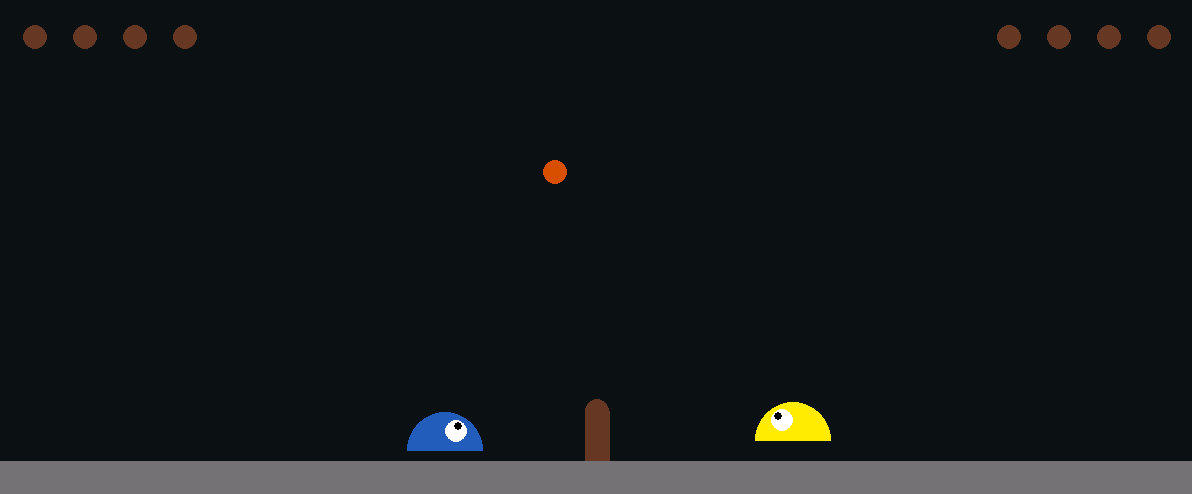
\includegraphics[width=0.9\textwidth]{img/slime-volleyball.png}
    \caption{Wizualizacja środowiska \texttt{SlimeVolley-v0}.}
    \label{fig:slime-volleyball}
\end{figure}

Celem agenta jest przebicie piłki przez siatkę w taki sposób, aby wylądowała ona na polu przeciwnika, co skutkuje utratą przez niego jednego z pięciu początkowych żyć. Epizod kończy się w momencie, gdy którykolwiek z graczy straci wszystkie życia, lub po upływie limitu 3000 kroków czasowych. Za każde życie odebrane przeciwnikowi agent otrzymuje nagrodę dodatnią (+1), natomiast utrata własnego punktu wiąże się z analogiczną karą (-1).

Agent podejmuje decyzje na podstawie obserwacji wektorów pozycji i prędkości obiektów w środowisku, a jego zadaniem jest opanowanie optymalnej strategii poruszania się. W ramach zaproponowanego podejścia proces uczenia realizowany jest poprzez bezpośrednią rywalizację z wcześniej wytrenowaną, ekspercką polityką bazową.

\section{Koncepcja rozwiązania}\label{sec:solution-concept}
Do rozwiązania problemu zastosowano podejście oparte na uczeniu ze wzmocnieniem (ang. \textit{Reinforcement Learning}), z wykorzystaniem algorytmu PPO (Proximal Policy Optimization) dostarczanego przez bibliotekę AgileRL~\cite{agilerl}. Uczenie agenta jest dodatkowo wspomagane ewolucyjną optymalizacją hiperparametrów (mutacje architektury i parametrów RL).

\subsection{Przestrzeń stanu i akcji}\label{subsec:state-action}
Stan środowiska (obserwacja) jest reprezentowany przez 12-wymiarowy wektor zawierający współrzędne położenia oraz wektory prędkości obu graczy i piłki z perspektywy agenta: $x_{ag}$, $y_{ag}$, $vx_{ag}$, $vy_{ag}$, $x_{ball}$, $y_{ball}$, $vx_{ball}$, $vy_{ball}$, $x_{opp}$, $y_{opp}$, $vx_{opp}$, $vy_{opp}$. Przestrzeń akcji to natomiast wektor \texttt{MultiBinary(3)}, co odpowiada jednoczesnemu sterowaniu ruchem w lewo, w prawo oraz skokiem.

\subsection{Składowe nagród}\label{subsec:reward-shaping}
Testy wykazały, że przyznawanie agentowi ciągłych nagród za samo odbijanie piłki prowadzi do wpadania w minima lokalne. Agent uczył się minimalizować kary, zamiast dążyć do zdobycia punktu. Zmodyfikowano więc środowisko, tworząc wariant \texttt{SlimeVolleyShaped-v0}. Wprowadzono w nim bardzo małą nagrodę o wartości 0.01 za przebicie piłki na połowę oponenta, co promuje aktywną grę. Ponieważ agenci potrafili zbyt długo podbijać piłkę po swojej stronie dodano zasadę, w której jeśli agent dotknie piłki więcej niż trzy razy z rzędu jest to traktowane jak strata punktu. Co ciekawe, wbudowana polityka bazowa nie znała tej zasady, ale jej styl gry i tak opierał się na wczesnych przebiciach nad siatką.

\subsection{Ekspercka polityka bazowa}\label{subsec:baseline-policy}
Przeciwnikiem w trakcie treningu była wbudowana polityka ekspercka~\cite{ha2015slimevolley}. Jest to mała rekurencyjna sieć neuronowa składająca się ze 120 parametrów. Została ona wcześniej wytrenowana od podstaw metodą uczenia przez grę przeciwko samemu sobie przy użyciu algorytmów genetycznych. Agenci rozgrywali ze sobą krótkie symulowane mecze bez żadnych zaprogramowanych heurystyk, optymalizując strategię wyłącznie na podstawie wygranych i przegranych.

\section{Architektura systemu}\label{sec:architecture}
System opiera się na algorytmie PPO, który jest stabilną metodą gradientową optymalizującą politykę aktora w trakcie gry. Działa on dobrze w tego typu problemach dzięki mechanizmowi przycinania funkcji celu, co zapobiega zbyt agresywnym aktualizacjom wag sieci podczas pojedynczego kroku uczenia. Parametry startowe, w tym współczynnik uczenia równy $3 \cdot 10^{-4}$ oraz rozmiar paczki danych wielkości 512, zostały dobrane na podstawie dokumentacji środowiska i własnych testów.

Ważnym elementem systemu jest wykorzystanie algorytmów ewolucyjnych. Podczas treningu na agentów w populacji nakładane są mutacje. Parametry uczenia mogą ulec zmianie z prawdopodobieństwem 30 procent, natomiast architektura samej sieci neuronowej ma szansę na zmianę struktury lub dodanie nowej warstwy. Pozwala to na automatyczne dostosowywanie modelu.

\section{Wyniki eksperymentów}\label{sec:results}
Trening wymagał przeprowadzenia dużej liczby kroków symulacji, przekraczającej 23 miliony iteracji dla całej populacji modeli. Wyniki i wykresy pokazują, że początkowa faza uczenia jest bardzo trudna, jednak model ostatecznie opanował grę w siatkówkę i zaczął regularnie pokonywać bazowego eksperta.

Najlepszy z wytrenowanych modeli zmodyfikował i powiększył swoją początkową architekturę sieci. Powstał w niej wspólny moduł przetwarzający dane wejściowe, składający się z trzech warstw liniowych o rozmiarach 64, 80 i 32 neuronów z zastosowaniem aktywacji ReLU. Optymalizacja ewolucyjna dostosowała też hiperparametry algorytmu: współczynnik uczenia spadł do około $9.8 \cdot 10^{-5}$, przetwarzana paczka danych wzrosła do 564, a rozmiar kroku środowiska ustalił się na poziomie 648.

Początkowe próby zrealizowania nauki zupełnie od zera przez grę własnych agentów przeciwko sobie okazały się na tym etapie zbyt czasochłonne obliczeniowo z wykorzystaniem metod jak IPPO (Independent Proximal Policy Optimization) dostępnych w bibliotece AgileRL. Możliwym kierunkiem na dalszy rozwój projektu byłoby zastąpienie oryginalnej polityki bazowej wytrenowanym agentem i ponowne uruchomienie procesu uczenia.

\begin{figure}[!htbp]
    \centering
    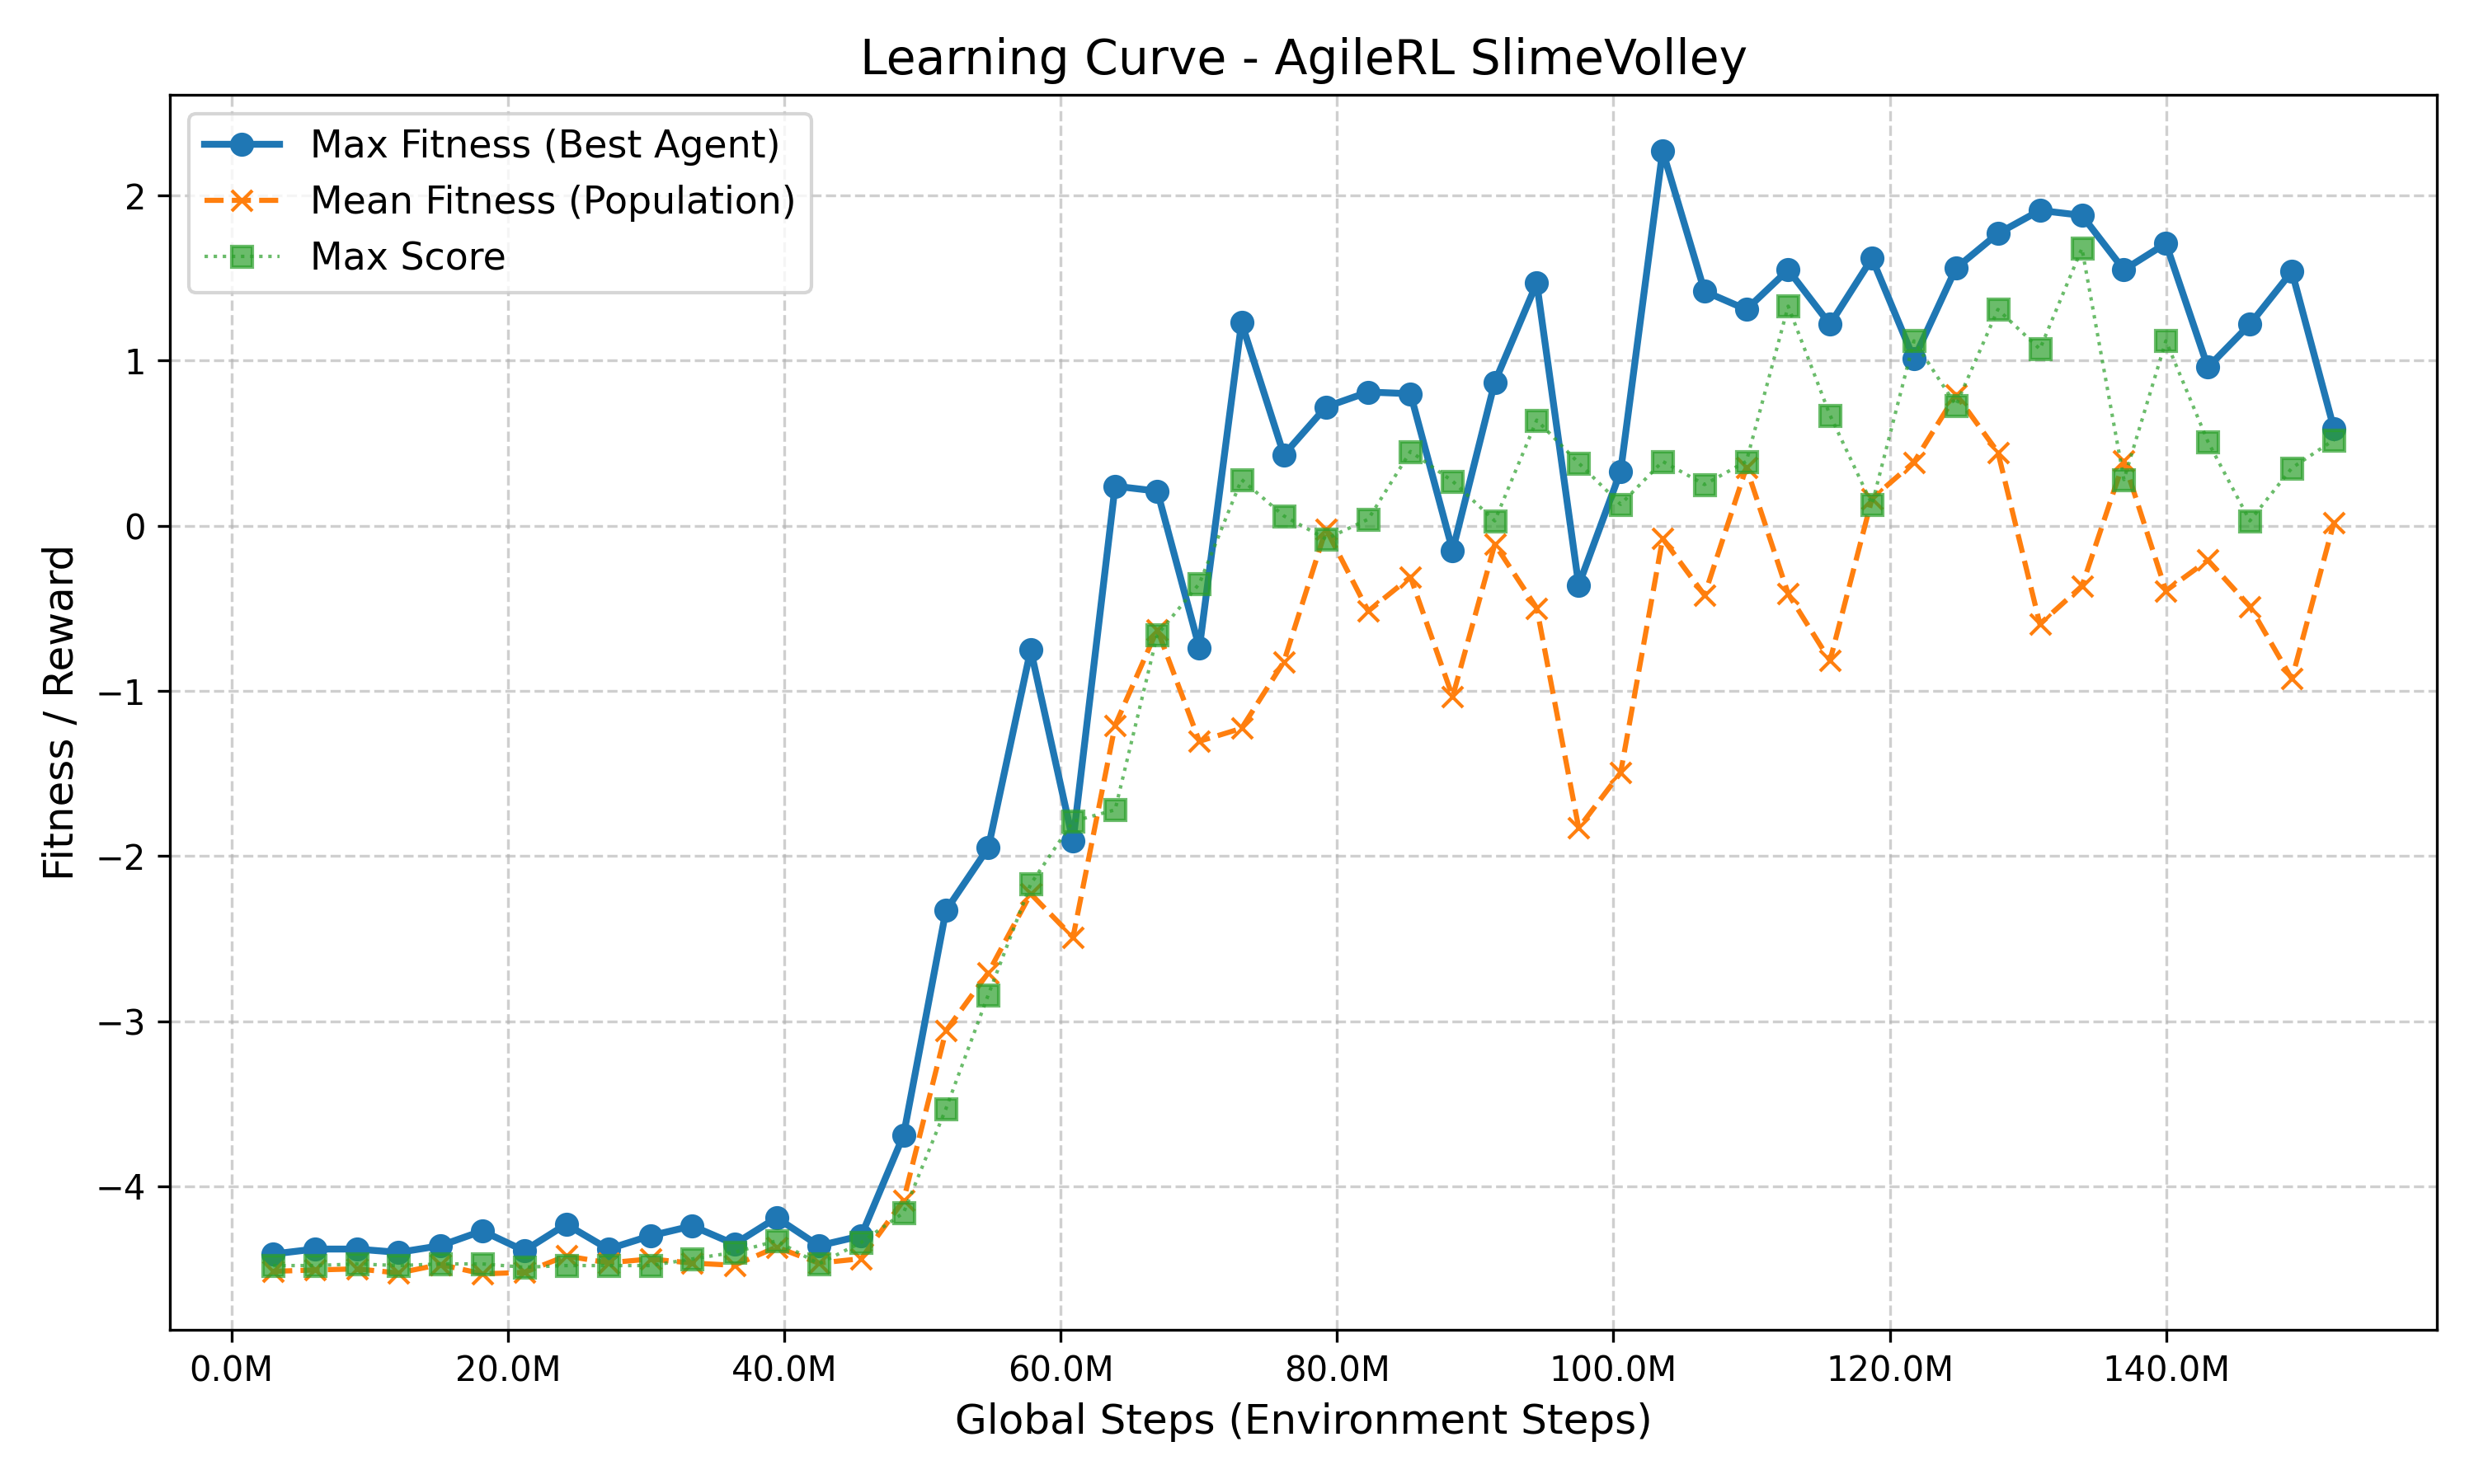
\includegraphics[width=0.9\textwidth]{img/learning-curve.png}
    \caption{Przebieg procesu uczenia algorytmu PPO z biblioteki AgileRL w środowisku \texttt{SlimeVolleyShaped-v0}.}
    \label{fig:learning-curve}
\end{figure}

\newpage
\bibliographystyle{plainurl}
\bibliography{bibliography}
